\documentclass{article}

% if you need to pass options to natbib, use, e.g.:
% \PassOptionsToPackage{numbers, compress}{natbib}
% before loading nips_2017
%
% to avoid loading the natbib package, add option nonatbib:

\PassOptionsToPackage{numbers, compress}{natbib}
\usepackage[final]{nips_2017}

% to compㅁle a camera-ready version, add the [final] option, e.g.:
\usepackage[utf8]{inputenc} % allow utf-8 input
\usepackage[T1]{fontenc}    % use 8-bit T1 fonts
\usepackage{hyperref}       % hyperlinks
\usepackage{url}            % simple URL typesetting
\usepackage{booktabs}       % professional-quality tables
\usepackage{amsfonts}       % blackboard math symbols
\usepackage{nicefrac}       % compact symbols for 1/2, etc.
\usepackage{microtype}      % microtypography
\usepackage{amsmath, amssymb, amsfonts, amsthm}
\usepackage[export]{adjustbox}
\usepackage{subcaption}
\usepackage[font=small]{caption}
\usepackage{todonotes}
%\usepackage[]{algorithm2e}
\usepackage{algorithm}
\usepackage[noend]{algpseudocode}
\usepackage{booktabs}

% Some reference styles
\newcommand{\eref}[1]{(\ref{#1})}% Equation
\newcommand{\aref}[1]{Algorithm~\ref{#1}}% Algorithm
\newcommand{\sref}[1]{Section~\ref{#1}}% Section
\newcommand{\figref}[1]{Figure~\ref{#1}}% Figure
\newcommand{\tabref}[1]{Table~\ref{#1}}% Table

\DeclareMathOperator*{\argmax}{arg\,max}
\DeclareMathOperator*{\argmin}{arg\,min}
\bibliographystyle{ieeetr}

\title{Bayesian-Adaptive Deep Reinforcement Learning using Model Ensembles}

% The \author macro works with any number of authors. There are two
% commands used to separate the names and addresses of multiple
% authors: \And and \AND.
%
% Using \And between authors leaves it to LaTeX to determine where to
% break the lines. Using \AND forces a line break at that point. So,
% if LaTeX puts 3 of 4 authors names on the first line, and the last
% on the second line, try using \AND instead of \And before the third
% author name.

\author{
  Gilwoo Lee \\ \texttt{gilwoo@cs.uw.edu} \\
  \And
  Jeongseok Lee \\ \texttt{jslee02@cs.uw.edu} \\
  \And
  Brian Hou \\ \texttt{bhou@cs.uw.edu} \\
  \And
  Aditya Mandalika \\ \texttt{adityavk@cs.uw.edu} \\
}

\begin{document}

\maketitle

% \begin{abstract}
% lalala abstract!
% \end{abstract}

\section{Introduction}
Although model-free deep reinforcement learning algorithms have shown tremendous success in a wide range of tasks, such as simulated control problems in OpenAI Gym~\cite{openai-gym} and games like Go~\cite{alphago}, they face fundamental challenges in their application to physical control problems on robotic hardware.
The high sample complexity of current methods results in long training periods if applied directly to hardware, even for simple grasping tasks~\cite{levine2016armfarm}.
Furthermore, the safety of the robot or surrounding environment when gathering data from the real world may be difficult to guarantee while the policy is training.

Model-based reinforcement learning techniques offer an opportunity to overcome these issues by taking advantage of simulations of the real systems, which can generate training data faster than real time.
The primary challenge with model-based techniques is the discrepancy between simulation and the real world.
Simplified models, inaccurate or uncertain parameters that govern the dynamics of the model, and other unmodeled disturbances and noise can render the policies learned on the simulated model ineffective on the real system.

We propose a model-based algorithm that learns a universal policy for Bayes-adaptive MDP that is robust and optimal to model uncertainty and disturbances. Although the real system's exact physical parameters are unknown, we can maintain a belief distribution over those parameters and provide this belief as an additional input to the policy.
This enables the learned policy to be bold when confident in its model and cautious when there is high model uncertainty.

\section{Related Work}
Our work is closely related to QMDP~\cite{littman1995learning, karkus2017qmdp} which is a Q-value approximation method for Partially Observable Markov Decision Processes (POMDPs).
QMDP assumes a fully-observable MDP after one action by approximating the Q-value at the current belief state $b(s)$ as a weighted average over the fully-observable MDP's Q-values $Q_a(b) = \sum_s b(s)Q_{\text{MDP}}(s, a)$.
The algorithm requires access to the (approximate) Q-function for the MDP.
QMDP performs surprisingly well for many problems, but determinizing the belief distribution after one timestep breaks Bayes-optimality.


%In our problem setup, we have a belief over the physics parameters $\phi$ of the MDP, $b(\phi)$, and we compute the policy $Q_a(s;b) = \sum_\phi b(\phi)Q_{\text{MDP}}(s,a;\phi)$.
%
The BAMDP formulation that we consider is also similar to the POMDP formulation used in POMDP-lite~\cite{chen2016pomdp}, which assumes that the hidden state variables remain constant or only change deterministically.
In our case, the hidden state variables correspond to the physics parameters $\phi$.
Chen et al. show that this formulation is ``equivalent to a set of fully observable Markov decision processes indexed by a hidden parameter'', which, in our case, is a discretization of $\phi$.

Robustness to model uncertainty has also been addressed by EPOpt~\cite{rajeswaran2016epopt}, which learns a policy that maximizes the worst-case performance across multiple sampled MDPs.
However, as is common with min-max techniques, EPOpt can be quite conservative (and therefore far from optimal) in its policy, especially when the model's possible parameter-space is large.
Our work closes this gap in EPOpt by maintaining a belief over the training MDPs to balance between optimality and robustness.

Another recent approach to model uncertainty is UP-OSI~\cite{yu2017uposi}, which utilizes online system identification to estimate the physical parameters of the system.
However, UP-OSI only uses the mean estimate of those parameters as an additional input to the policy.
Without a notion of belief and uncertainty in its parameter estimates, UP-OSI is prone to aggressively executing policies without being conservative toward remaining model uncertainty.

TODO: mention \cite{guez2014bayes} and other bayesian work.

\section{Bayes-Adaptive Reinforcement Learning}

\begin{figure*}[t!]
\centering
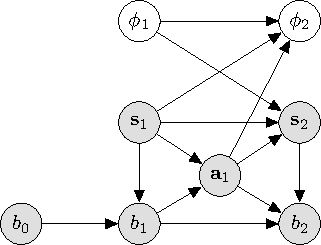
\includegraphics[width=0.5\linewidth]{figs/model.pdf}
\caption{Graphical model for a Bayes-Adaptive Markov Decision Process.}
\label{fig:pgm}
\end{figure*}

We follow the Bayes-Adaptive Markov Decision Process framework (\figref{fig:pgm}), which assumes that a latent variable $\phi$ governs the transition function of the underlying Markov Decision Process~\cite{ghavamzadeh2015bayesian, ross2008bayes, guez2012efficient}.
A Bayes-Adaptive MDP is defined by a tuple $\langle \mathcal{S}', \mathcal{A}, P, P_0, R \rangle$, where
\begin{itemize}
\item $\mathcal{S'} = \mathcal{S}\times \Phi$ is the set of hyper-states (state $s$, latent variable $\phi$),
\item $\mathcal{A}$ is the set of actions,
\item $P(s',\phi'|s, \phi, a)$ is the transition function between hyper-states, conditioned
on action $a$ being taken in hyper-state $(s, \phi)$,
\item $P_0\in \mathcal{P}(\mathcal{S} \times \Phi)$ combines the initial distribution over hyper-states,
\item $R(s, \phi, a)$ represents the reward obtained when action $a$ is
taken in hyper-state $(s,\phi)$.
\end{itemize}
In our setting of robot control, the latent variables $\phi$ are physics parameters such as mass and length of different robot links (TODO: better word than links) (JS: robot bodies?).

Our goal is to find the Bayes-optimal policy for the following Bellman equaton:
\begin{equation}\label{eq:rl}
V^*(b, s) = \max_a \bigg\{R(s, b, a) + \gamma \sum_{s'}P(s', b'|s, b, a)V^*(b', s') \bigg\}.
\end{equation}
where $b(\phi)$ is the belief over the set of latent physics parameters $\phi \in \Phi$,
\begin{align*}
R(s, b, a)
  &= \sum_{\phi \in \Phi} b(\phi) R(s, \phi, a) \\
P(s', b' | s, b, a)
  &= \sum_{\phi \in \Phi} b(\phi) P(s', b' | s, \phi, a) \\
  &= \sum_{\phi \in \Phi} b(\phi) P(s' | s, \phi, a) \sum_{\phi' \in \Phi} P(\phi' | s, \phi, a)
\end{align*}

TODO(?): mention PAC-MDP?

\subsection{Belief Update}

We make a simplification to the BAMDP formulation by assuming that the latent variable $\phi$ is constant or changing deterministically according to a known transition function.
% \footnote{
% A looser assumption is that the rate of change of $\phi$ is slow enough that approximating the long-term value with the same $\phi$ is a reasonable short-term approximation for choosing the one-step action, i.e. we can treat $V^*(s_t, \phi_t) \approx V^*(s_t, \phi_{t:\infty})$ for a one-step Bellman update.
% }
As in POMDP-lite\cite{chen2016pomdp}, we can then view the simplified BAMDP model as a set of MDPs that are indexed by the latent variable $\phi$.

% \begin{align*}
% b(\phi_t) = P(\phi_t|s_{t-1}, \phi_{t-1}, a_{t-1})
% \end{align*}
% which is then used to compute the best policy from an ensemble of $\phi$-dependent optimal policies, i.e., $\pi^*(\cdot;\phi)$ and $V^*(\cdot;\phi)$ are computed with typical RL algorithms for MDPs.
% Then the remaining task is to compute the one-step best action $a$:
% \begin{align}\label{eq:barl}
%  a^* &= \argmax_{a} \mathbb{E}_{\phi \sim b(\phi)} \bigg[R(s, a, \phi) + \gamma \sum_{s', \phi'}P(s',\phi'|s, \phi, a)V^{*'}(s', \phi') \bigg].
% \end{align}

The posterior probability of an MDP governed by latent physics variable $\phi$ given a trajectory $\tau_{0:H} = (s_0, a_0, \cdots, s_H)$ is given by:
\begin{align}
P(\phi_H | \tau_{0:H})
  &= \frac{1}{Z} P(\phi_0) P(\tau_{0:H} | \phi_0) \nonumber \\
  &= \frac{1}{Z} P(\phi_0) \prod_{t=0}^{H-1} P(s_{t+1}, \phi_{t+1} | s_t, \phi_t, a_t) \nonumber \\
  &= \frac{1}{Z} P(\phi_0) \prod_{t=0}^{H-1} P(s_{t+1}|s_t, \phi_t, a_t) P(\phi_{t+1} | s_t, \phi_t, a_t)
\end{align}
where $Z$ is a normalizing constant and $P(\phi_{t+1} | \cdot) = 1$ is the deterministic transition of $\phi$.

% Assuming that $\phi$ is constant allows us to simplify the belief update rule at each timestep $t$:
% \begin{align*}
% b_t(\phi) \propto \sum_{\phi \in \Phi} P(\phi|s_{t-1}, a_{t-1}) b_{t-1}(\phi)
% \end{align*}
% Our algorithm uses the state augmented with this updating belief as the input to the policy at each timestep.

\section{Bayes-Adaptive Policy Gradient}

\begin{figure*}[t!]
\centering
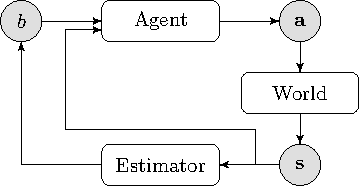
\includegraphics[width=0.5\linewidth]{figs/system_structure.pdf}
\caption{System structure}
\end{figure*}

The main contribution of our work is a policy-gradient algorithm which produces a universal policy that maintains different strategies for different beliefs. The key idea is to augment the state with the belief and provide this augmented feature as input to the policy. The policy is a function of both state and belief: $\pi: \mathcal{S} \times \mathcal{B} \rightarrow P(\mathcal{A})$, where $\mathcal{B}$ is the belief space. This allows the policy to differentiate between the beliefs while sharing globally effective strategies.

In order for this algorithm to work in practice, we need an effective representation of the belief space. If the space of MDPs, $\mathcal{M}$, is finite, the belief $b$ can be a vector of size $|\mathcal{M}|$. In case where $\mathcal{M}$ is infinite, we propose two methods to approximate the belief space:

\begin{itemize}
    \item Sample $K$ MDPs from the prior belief distribution $b_0$ and use belief over these $K$ MDPs
    \item Discretize the parameter space and use belief over the parameter space
\end{itemize}
In the first case, we use a vector of size $K$ as $b$; $K$ should be large enough to approximate all MDPs with the K sampled ones. In the second case, assuming the latent parameters are independent, the belief is represented as a vector of size $(N_1 + .... + N_M)$ where $M$ is the total number of parameters and $N_m$ is the discretization of the $m$-th parameter. In this project we have implemented the first one, and leave the second one as future work.

The algorithm is shown in \aref{algo:bapg}. At each iteration, we sample a number of MDPs from the prior distribution $b_0$, and sample a trajectory for each MDP using the latest policy. During the rollout of the trajectory, the estimator provides the updated belief estimate as an additional feature to the policy. The estimator resets to $b_0$ at the beginning of each trajectory.

Note that the policy observes the \emph{evolution} of belief along each trajectory. This allows the policy to learn to be optimal with respect to the evolution of belief, and to take actions which affect the evolution. For example, given prior belief $b_0$ with high entropy (i.e., high uncertainty), our algorithm policy would produce conservative or informative actions until $b$ becomes informative enough along the course of the trajectory. This is a key difference between our algorithm and \cite{yu2017uposi}, in which the policy has no notion of belief or uncertainty.

%%\newcommand{\argmin}{\operatornamewithlimits{\arg\min}}
%
%
%------------------------------------------
% Algorithm:
%------------------------------------------%
\begin{algorithm}[tb]
\caption{\texttt{Bayes-Adaptive Policy Gradient}}
\label{algo:bapg}
\begin{algorithmic}[1]
\State Bayes-Estimator $ES$, $b_0$, $\theta_0$, $n_\text{itr}$, $n_\text{sample}, \mathcal{M}$\Comment{Initialization}
\vspace{2mm}
\For{i = 1, 2, ..., $n_\text{itr}$}
  \For{n = 1, 2 , ..., $n_\text{sample}$}
    \State Reset $ES$ with $b_0$
    \State Sample model parameter $\phi \sim b_0$ to get $M_{\phi}$
    \State Sample a trajectory $\tau_n$ from $M_{\phi}$ using policy $\pi(\theta_i)$ and estimator $ES$
  \EndFor
\EndFor
\State Update policy: $\pi(\theta_{i+1}) = \texttt{BatchPolOpt}(\theta_i, \{\tau_1, ..., \tau_{n_{sample}}\})$
\end{algorithmic}
\end{algorithm}

\section{Experiments}

Our algorithm falls under the class of model-based algorithms that consider multiple MDPs to train a policy. We therefore compare our algorithm against (1) QMDP and (2) EPOpt. QMDP makes the assumption that $\phi$ is revealed after one step, and takes the best action given $b(\cdot)$, i.e. $a^* = \max R(s,b,a) + \sum_{\phi\in\Phi} b(\phi)Q(s,a,\phi)$. EPOpt is a minimax-style algorithm which trains the policy to be robust across multiple MDPs, without utilizing the belief over MDPs in learning the policy.

We evaluate the three algorithms on a set of simulated benchmark examples: ant (TODO cite), swimmer (TODO cite) and the half-cheetah (TODO cite) using the MuJoCo physics simulator (TODO cite). 
Owing to the numerous model parameters that can be varied to simulate multiple possible MDPs, these benchmarks prove to be ideal to test robustness against model discrepancies (TODO: refer the tables). 
Each of the agents is provided a pre-defined reward function as in OpenAI Gym ~\cite{openai}. 

For each agent, we uniformly sampled 20 MDPs across a range of parameters as in (TODO: refer the table) (e.g., body link length, mass, geometry size, joint damping, friction), and used these as the set of MDPs with which we approximate the belief space.

We implemented EPOpt as in \cite{rajeswaran2016epopt} with TRPO \cite{trpo} provided by \texttt{rllab}~\cite{duan2016benchmarking} as the underlying batch policy optimization sub-routine.
Our implementation of QMDP uses TRPO policies trained on the chosen 20 MDPs to rollout trajectories and approximate Q-functions. EPOpt

All policy networks were Gaussian MLPs with two layers, (64, 64), except for Bayes ones which had (128, 64) to account for the larger input space.

\begin{itemize}
    \item By augmenting the observation with a belief over  MDPs, policy networks can learn to be robust against    model uncertainty while maintaining some of the
    ``optimal'' actions w.r.t. each MDP.
    \item When the optimal policies across MDPs have a lot in   common (e.g., Swimmer), simple "interpolation" of the deterministic policies provide good action proposals,
    suggesting that a mixture of policies (with a large number of policies that cover the space), may reduce sample complexity and offer even better performance.
\end{itemize}

\begin{table}[ht]
\caption{Model Parameters}
\centering
\begin{tabular}{l c c c c} % centered columns (4 columns)
\hline\hline %inserts double horizontal lines
Parameter & $\mu$ & $\sigma$ & Low  & High \\ [0.5ex] % inserts table
%heading
\hline % inserts single horizontal line
\rule{0pt}{2ex}  
Mass & 1 & 50 & 837 & 970 \\ % inserting body of the table
Friction & 2 & 47 & 877 & 230 \\
Damping & 4 & 35 & 144 & 2356 \\
Deadpool & 5 & 45 & 300 & 556 \\ 
Front-Link-Length & 3 & 31 & 25 & 415 \\ [1ex] % [1ex] adds vertical space
\hline %inserts single line
\end{tabular}
\label{physicsParams}
\end{table}


%
%\begin{figure*}[t!]
%\begin{centering}
%\begin{subfigure}[b]{0.24\columnwidth}
%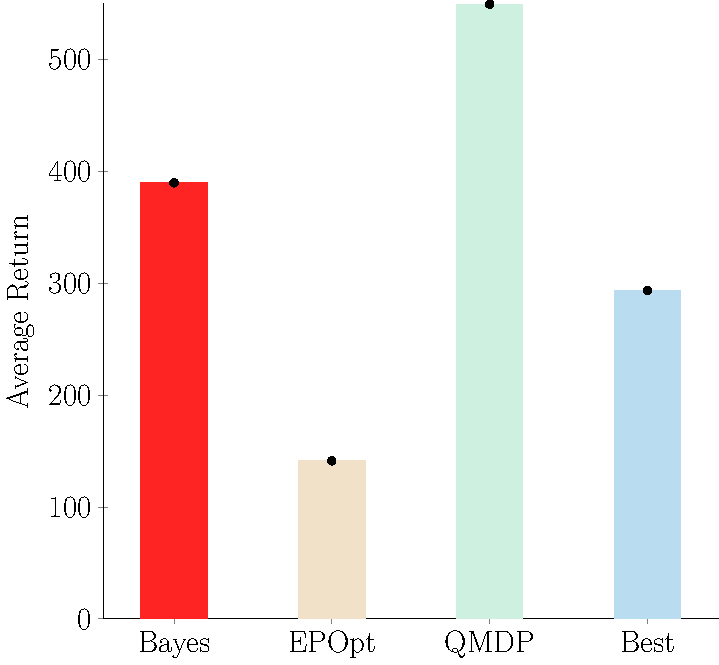
\includegraphics[width=\linewidth]{figs/cheetah_nominal_comparison.pdf}
%\subcaption{Nominal MDP}
%\end{subfigure}
%~
%\begin{subfigure}[b]{0.24\columnwidth}
%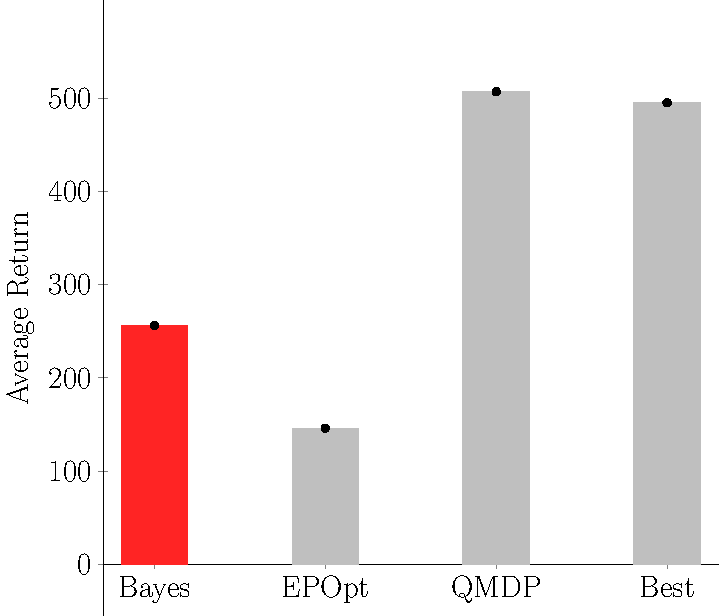
\includegraphics[width=\linewidth]{figs/cheetah_env_comparison.pdf}
%\subcaption{One of K MDPs}
%\end{subfigure}
%~
%\begin{subfigure}[b]{0.22\columnwidth}
%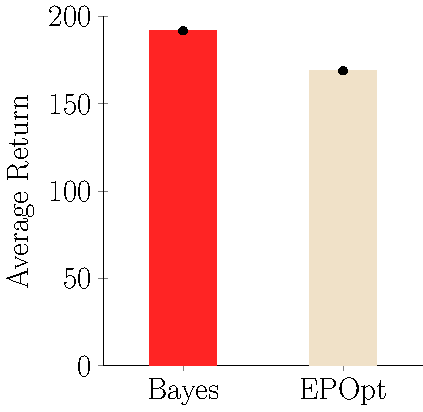
\includegraphics[width=\linewidth]{figs/cheetah_average.pdf}
%\subcaption{Over 20 MDPs}
%\end{subfigure}
%\end{centering}
%\caption{Return on sampled and prechosen MDPs. BARL is better than EPOpt. On average across K pre-chosen MDPs, it outperforms EPOpt by a large margin. TODO: remove BMP.}
%\end{figure*}



\section{Future Work}

\begin{itemize}
    \item Extend to a continuous version which has Gaussian belief distribution as input
    \item Bootstrap a set of stochastic/deterministic policies, each trained for one MDP or a small range of parameters
    \item Train with additional reward bonus for information gain which helps distinguishing policies (not just beliefs)
\end{itemize}


\begin{figure*}[t!]
\begin{centering}
\begin{subfigure}[b]{0.3\columnwidth}
\adjincludegraphics[height=3cm,trim={{.6\width} {0.4\height} {0.15\width} {0.35\height}},clip=true]{figs/keyframes/cheetah/cheetah_nominal.png}
\caption{Nominal}
\end{subfigure}
\begin{subfigure}[b]{0.3\columnwidth}
\adjincludegraphics[height=3cm,trim={{.5\width} {0.4\height} {0.25\width} {0.35\height}},clip=true]{figs/keyframes/cheetah/cheetah_170_92.png}
\caption{Key frames}
\end{subfigure}
\begin{subfigure}[b]{0.3\columnwidth}
\adjincludegraphics[height=3cm,trim={{.5\width} {0.4\height} {0.25\width} {0.35\height}},clip=true]{figs/keyframes/cheetah/cheetah_150_150.png}
\caption{Key frames}
\end{subfigure}
\begin{subfigure}[b]{0.3\columnwidth}
\adjincludegraphics[height=3cm,trim={{.4\width} {0.42\height} {0.35\width} {0.33\height}},clip=true]{figs/keyframes/ant/ant_nominal_18.png}
\caption{Nominal}
\end{subfigure}
\hfill
\begin{subfigure}[b]{0.3\columnwidth}
\adjincludegraphics[height=3cm,trim={{.4\width} {0.42\height} {0.35\width} {0.33\height}},clip=true]{figs/keyframes/ant/ant_120_19.png}
\caption{Key frames}
\end{subfigure}
\hfill
\begin{subfigure}[b]{0.3\columnwidth}
\adjincludegraphics[height=3cm,trim={{.6\width} {0.34\height} {0.15\width} {0.41\height}},clip=true]{figs/keyframes/ant/ant_140_87.png}
\caption{Key frames}
\end{subfigure}
\vfill
\begin{subfigure}[b]{0.3\columnwidth}
\adjincludegraphics[height=3cm,trim={{.55\width} {0.34\height} {0.20\width} {0.41\height}},clip=true]{figs/keyframes/swimmer/swimmer_nominal.png}
\caption{Nominal}
\end{subfigure}
\hfill
\begin{subfigure}[b]{0.3\columnwidth}
\adjincludegraphics[height=3cm,trim={{.55\width} {0.40\height} {0.20\width} {0.35\height}},clip=true]{figs/keyframes/swimmer/swimmer_20_12.png}
\caption{Key frames}
\end{subfigure}
\hfill
\begin{subfigure}[b]{0.3\columnwidth}
\adjincludegraphics[height=3cm,trim={{.35\width} 0 {0.40\width} {0.55\height}},clip=true]{figs/keyframes/swimmer/swimmer_40_157.png}
\caption{Key frames}
\end{subfigure}
\end{centering}
\caption{Keyframes from rollouts on various MDPs. Some of the MDPs are gemeotrically significatnly differnt that they require drastically different policies to achieve optimal returns.}
\end{figure*}

\bibliography{intuitive_physics}

\end{document}
